\chapter{Reflectometry Measurements of the Loss Tangent in Silicon at Millimeter Wavelengths}
\label{ch:si}
The following was published in the proceedings from the 8th ESA Workshop on Millimetre-Wave Technology and Applications in 2018~\cite{ches18}.
\section{Introduction}
Dielectric loss and its associated thermal emission is a key driver for sensitivity in millimeter wave receivers. A low loss implies low emission from a material, therefore limiting thermal noise propagating through to the detector. The
contribution to the thermal noise due to loss,  $T_{\text{sys}}$, can be calculated as:
\begin{equation}
    T_{\text{sys}}=T_{\text{comp}}(L-1)
\end{equation}
where $T_{\text{comp}}$ is the physical temperature of the component, $L=\exp(2\pi n \tan(\delta)/\lambda_0)$ is the optical loss, $n$ is the index of refraction, $\tan(\delta)$ is the loss tangent, $t$ is the sample thickness, and $\lambda_0$ is the free-space wavelength. The noise due to loss can be reduced in two ways: lowering the temperature of the component, and using materials with lower intrinsic loss. 

Many millimeter wave experiments use cold optical components to minimize noise contributions due to this thermal
emission. However, in many cases, it is advantageous to include warm silicon components in optical designs. For example,
in the ALMA Band 1 receivers include a warm lens that also acts as the window into the cryostat. The original design
uses a plastic (high density polyethylene) lens that contributes one-third of the overall receiver noise budget. Substitution of a lens with lower dielectric losses could therefore make a substantial impact on the sensitivity of this instrument.

Silicon is a potentially attractive material for such applications. Datta et al. 2013 showed that silicon can be machined to produce very high quality anti-reflective (AR) meta-surfaces to reduce the reflected power from the natural 30\% to levels in the few tenths of a percent range~\cite{Datta:13}. The key development required is identification of a source of silicon with low dielectric losses at room temperature.

Since it was first reported in Parshin et al.~\cite{parshin} and included in the Lamb 1996 compendium of mm-wave material properties~\cite{lamb}, the promise of silicon as an intrinsically low-loss mm/sub-mm optical material has tantalized the astronomical community.   More recently, Krupka et al. 2016~\cite{KRUPKA201676} reported on the result of a loss tangent in Ka-band and Q-band ($\approx27-40$\,GHz) on the order of $\tan(\delta)\lesssim 10^{-5}$ at room temperature ($\approx300\,K$) for samples of proton-irradiated high purity FZ silicon, but measurements in W-band ($\approx$90\,GHz) and for neutron-irradiated samples are lacking. We address this here using coherent reflectometry measurements.

\section{Procedure}
\subsection{Optical Hardware}
A feedhorn source sends a millimeter wave signal to a parabolic mirror, which sends a plane wave toward the sample, typically at a 10$^{\circ}$ angle of incidence. For these measurements, the sample is a dielectric slab immersed in air. A portion of the signal is reflected to the first air-dielectric boundary, and the remaining signal propagates through the sample, where it again partially reflects from the second dielectric-air boundary, leading to a Fabry-Perot interference in the dielectric cavity defined by the sample. The reflected signal propagates to a second mirror, followed by the receiver feed horn. The geometry is shown in Figure~\ref{fig:optical_setup}.

Eccosorb is placed on surfaces outside the beam in order to reduce and absorb unwanted reflections.   The alignment of the receiver is controlled with a three-axis stage. The tilt of the sample is controlled with a three-point micrometer mount.   This angle is chosen by placing an aluminum plate in the sample holder and maximizing the received signal at a single frequency. Once the setup is aligned, a calibration data set is taken by measuring the reflectance of the aluminum plate as a function of frequency. This dataset serves to define perfect reflection.   The aluminum plate is then replaced with the sample (silicon here) and the measurement is made. The response of the silicon sample measurement is divided by the response of the aluminum plate to yield a measurement of the reflectance of the sample as a function of frequency.

\subsection{Receiver Electronics}
A correlation receiver designed for a holography system is used for these measurements. The receiver compares a reference signal to a signal which has passed through the device, creating an interference pattern between the two.   The holographic imaging setup is summarized in Figure~\ref{fig:holog_ref_setup}.   The Re-configurable Open Architecture Computing Hardware (ROACH2) board correlates the reference and modulated signals~\cite{roach2}.

\subsection{Samples: Neutron-irradiated and Intrinsic Silicon}
Two samples were provided by Topsil for testing. The samples as cut exhibited curvature and uneven thickness of approximately 15\,mm. A professional third party was contracted to grind and polish the samples flat and parallel. The
resulting thicknesses are reported in Table 1, and are accurate to scales $\ll \lambda_0$ measured with a micrometer. The silicon is made with Float Zone mono growth in an oxygen-free environment, reducing risk of generating thermal donors during
high temperature processes~\cite{topsil}.
\section{Reflectometry and Transmissivity}
We measured the transmission and reflection of these samples. The data are shown in Figure~\ref{fig:si_data}.
\begin{figure}[t]
    \centering
    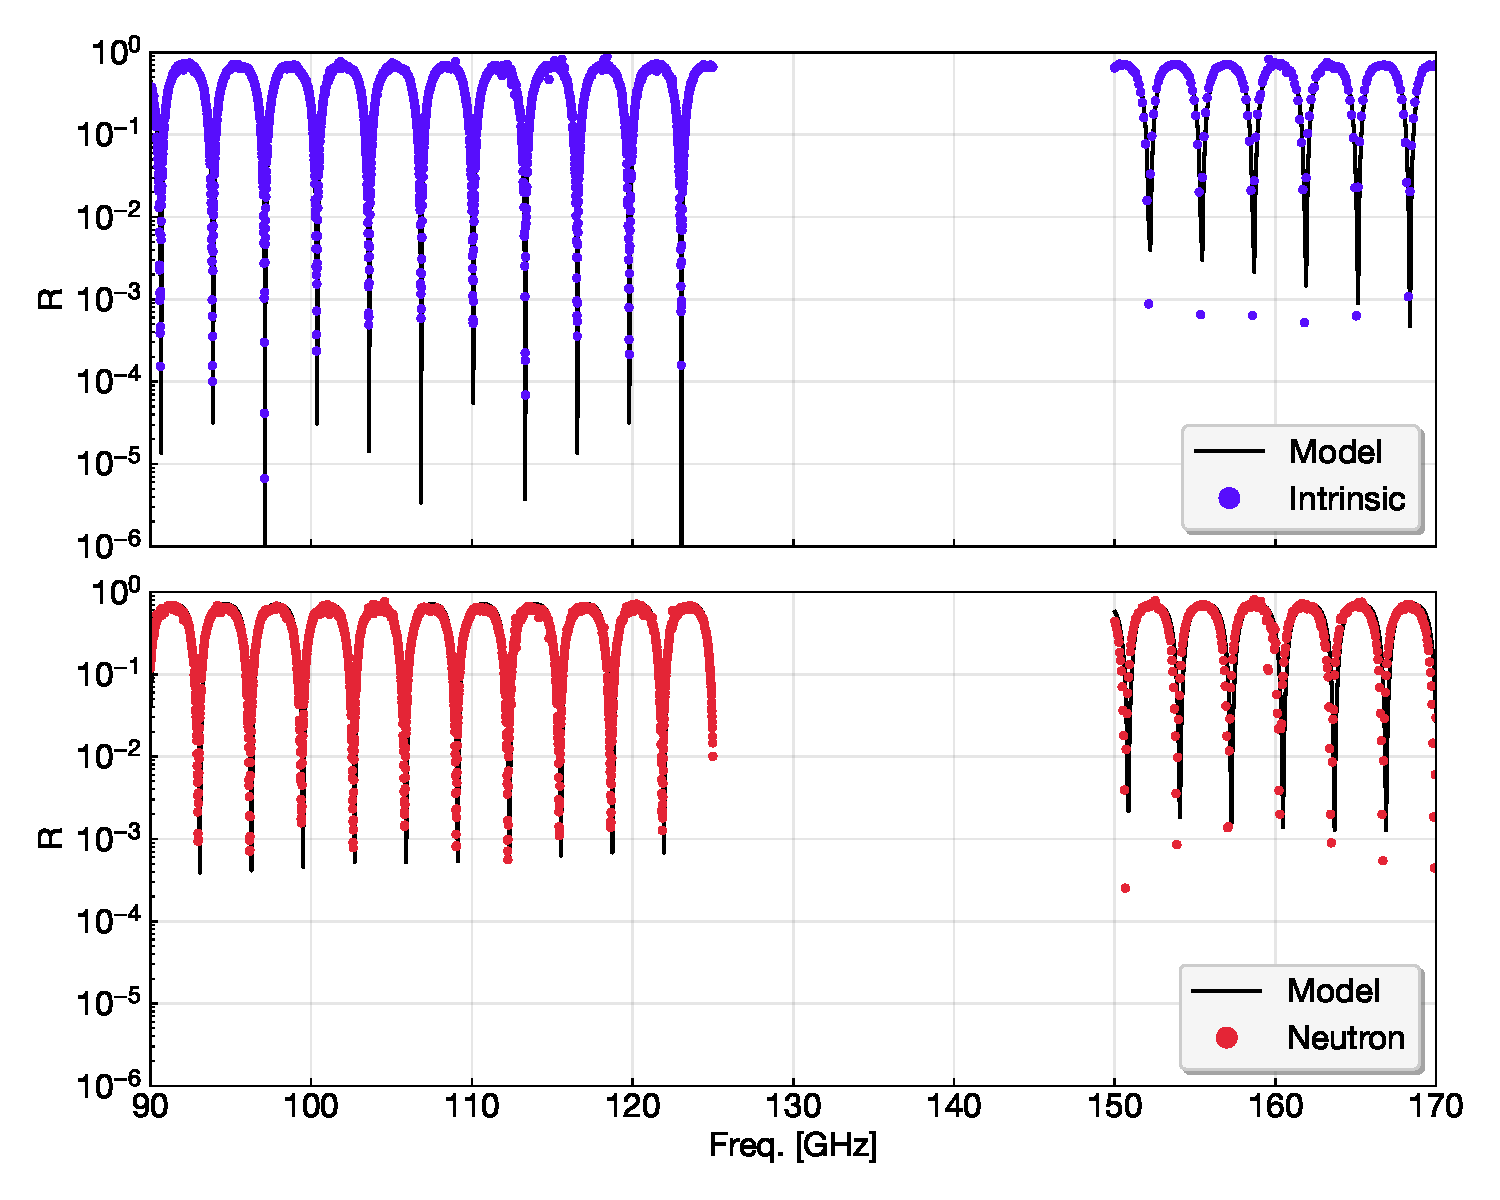
\includegraphics[width = .9\textwidth]{Figures/silicon_refl.pdf}
    \caption{Reflectivity of intrinsic (top) and neutron-irradiated (bottom) silicon against frequency [GHz].}
    \label{fig:si_data}
\end{figure}
\subsection{Modeling}
We model the dielectric slab with a complex index $n_2 = n_r + in_i$.  Air is treated with a purely real index $n_1 = $. The refracted angle in each layer is calculated using Snell's law, where $\theta_1$ is the incident angle and $n_1$ is the free-space
index of the first layer (i.e. $n_1$ in Eq.~\ref{eq:snell}). The setup began at an incidence angle of $10^{\circ}$.

\begin{equation}
    \theta_2 = \arcsin\bigg(\frac{n_1}{n_2}\sin\theta_1\bigg)
    \label{eq:snell}
\end{equation}
The experiment exclusively uses TM mode signals, where the reflected and transmitted coefficients theoretically
predicted by~\cite{jackson}:

\begin{equation}
    R = \frac{n_1 \cos\theta_2 - n_2\cos\theta_1}{n_1\cos\theta_2 + n_2\cos\theta_1}
    \label{eq:R_snell}
\end{equation}

\begin{equation}
    T = \frac{2 n_1 \cos\theta_1}{n_2\cos\theta_1 + n_1\cos\theta_2}
    \label{eq:T_snell}
\end{equation}

\begin{equation}
    \tan(\delta) = 2n_i/n_r
    \label{eq:loss}
\end{equation}

Using Eq.~\ref{eq:R_snell} and Eq.~\ref{eq:T_snell}, where the parameter $n_2$ is the fitting parameter, the material index is extracted from measurements. 

\subsection{Fitting}
the loss tangent (or equivalently complex part of the index) leads to a reduction in the depth of the reflection nulls for this signal. The cancellation of the incident and reflected waves is more perfect for lower loss tangent. Therefore, the nulls in the reflection are crucial to get a reliable constraint on the loss. We also note that one of the dominant systematic effects is standing waves between the source and receiver horn. This systematic includes a reflection from the sample. Therefore, this noise is minimized near the nulls. For this reason, we fit the data only where the reflectance is below some threshold (typically $R<0.01$, though, varying this by a factor of a few has no impact on the results). The weighing of each data point scales as the inverse of reflectivity to force the fit to focus on the depth of the nulls. We test that the analysis doesn’t depend on this weighting by doing describe. We implemented a Markov Chain Monte Carlo algorithm for fitting the reflectivity model to our measurements using the Python package \verb|pyMC|, with the real and imaginary components of the index of refraction as fitting parameters~\cite{Patil2010PyMCBS}. The Markov Chain Monte Carlo algorithm samples the probability distribution of each parameter, in this case the probability of two parameters in the reflectivity model matching the measured reflectivity of the sample. This method was used to fit the measurement to the model, yielding, the real and imaginary components of index of refraction of the sample. The loss, $\tan(\delta)$, of the material is then calculated using Eq.~\ref{eq:loss}.

The error bars of loss values are calculated with two methods. The first method is the MCMC error computation with the \verb|pyMC| package in Python. To check these values, each null is fit individually using the MCMC algorithm, yielding an array of parameter values. The root-mean-square (RMS) of these values is then calculated, yielding the RMS error. Both methods yielded nearly equivalent loss error results, and we therefore report the MCMC loss error in Table~\ref{tab:silicon}. The error in index of refraction is not reported as it is likely included in the uncertainty of the thickness, while the MCMC reported a negligible error for this parameter.

\begin{table}
    \centering
\begin{tabular}{ |p{3cm}|p{3cm}|p{3cm}| }
 \hline
 Silicon & Neutron & Intrinsic\\
 \hline
  $n$ & 3.415 & 3.412 \\
 \hline
 $\tan(\delta)\times 10^{-5}$ & $28.93 \pm 1.21$ & $1.47 \pm 0.09$\\
 \hline
  D\,[mm] & $13.68 \pm 0.1 $ & $13.56 \pm 0.1$\\
 \hline
\end{tabular}
    \caption{Optical properties of silicon. Properties extracted from the data when fit with the theoretical model. Properties $n$ is the index of refraction, D is the thickness of the sample, and $\tan(\delta)$ is the loss tangent.}
    \label{tab:silicon}
\end{table}

\section{Results}

The index of refraction of neutron and intrinsic silicon are nearly identical, with $n =3.415$ for neutron-irradiated silicon, and $n =3.412$ for the intrinsic silicon samples. The neutron-irradiated sample has $\tan(\delta) = 2.8\times10^{-4}$, while the intrinsic silicon is nearly an order of magnitude better, with $\tan(\delta)= 1.5 \times 10^{-5}$. See Table~\ref{tab:silicon} for a summary of the measured and inferred properties.

The reason for the higher loss in the neutron-irradiated sample is unclear, as the loss tangent should improve for materials with higher resistivity if dominated by the conduction loss term. As the resistivities of the neutron-irradiated and unmodified intrinsic silicon samples were measured by Topsil to be $>100\,k\Omega-cm$ and $>50k\,\Omega-cm$, respectively, the expectation is that the neutron-irradiated sample should have less loss. One possible explanation is that the lattice defects introduced by neutron irradiation contribute to the loss.

The resulting values for $\tan(\delta)$ from fits to our measurements of the unmodified intrinsic silicon sample are comparable to those reported in Parshin et al. 1995~\cite{parshin}. Further, our measured low loss in intrinsic silicon demonstrates it can be a compelling material for use in warm optics. Krupka et al.~\cite{KRUPKA201676} also report a $\tan(\delta) \approx 1.2\times10^{-5}$ for proton-irradiated silicon, which is lower by more than $3\sigma$ than our measurements of intrinsic silicon, but on the same order of magnitude. Our work shows promise for the use of intrinsic silicon for room-temperature optical components, such as those required for the lower bands of the Atacama Large Millimeter/Sub-millimeter Array (ALMA) and potential future CMB experiments.


